\documentclass{article}

\usepackage{
    amsmath
,   physics
,   microtype
,   graphicx
,   enumitem
,   gensymb
,   tikz
,   color
,   etoolbox
,   fancyhdr
}
\usepackage[letterpaper, top=1in, bottom=1in, left=1in, right=1in]{geometry}

\pagestyle{fancy}

\patchcmd\subequations{\alph}{\Alph}{}{}{}
\usepackage{hyperref}

\title{Kinematic Practice Problems}
\author{Laith Toom}
\date{24/2/2023}

\begin{document}
\maketitle
\newpage
\tableofcontents
\newpage

\section{Chapter 2: 1D Motion}

    \subsection{Problem 34: Page 34}
    A red car and a green car, identical except for the 
    color, move toward each other in adjacent lanes and 
    parallel to an $x$ acis. At time $t=0$, the red car 
    is at $x_r=0$ and the green car is at $x_g=200\,\mathrm{m}$.
    If the red car has a constant velocity of $20\,\mathrm{km/h}$,
    the cars pass each other at $x=44.5\,\mathrm{m}$, and if it has 
    a constant velocity of $40\,\mathrm{km/h}$, they pass each other at
    $x=76.6\,\mathrm{m}$. What are:
    \begin{enumerate}[label=(\alph*)]
        \item the initial velocity 
        \item the constant acceleration
    \end{enumerate}
    of the green car?
    \begin{figure}[h!]
        \centering 
        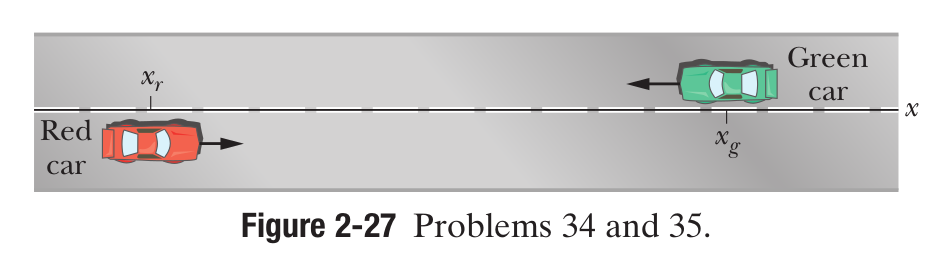
\includegraphics[width=10cm]{Exam1Practice_Figures/fig34_34.png}
    \end{figure}
    \begin{subequations}

    \subsubsection{Solution}
    \end{subequations}

\newpage

\section{Chapter 3: Vectors}

    \subsection{Problem 29: Page 58}
    Typical backyard ants often create a network of chemical 
    trails for guidance. Extending outward from the nest, a trail
    branches (\textit{bifurcates}) repeatedly, with $60\degree$
    between the branches. If a roaming ant chances upon a trial, it 
    can tell the way to the nest at any branch point: If it is moving 
    awat from the nest, it has two choices of path requiring a small turn 
    in its travel direction, either $30\degree$ leftward or $30\degree$
    rightward. If it is moving toward the nest, it has only one such choice. 
    Figure 3-29 shows a typical ant trial, with lettered straight sections
    of $2.0\,\mathrm{cm}$ length and symmetric bifurcation of $60\degree$.
    Path $v$ is parallel to the $y$ axis. What are the:
    \begin{enumerate}[label=(\alph*)]
        \item magnitude
        \item angle
    \end{enumerate}
    (relative to the positive direction of the superimposed $x$ axis) of 
    an ant's displacement from the nest (find it in the figure) if the ant 
    enters the trail at point $A$? What are the:
    \begin{enumerate}[label=(\alph*), start=3]
        \item magnitude
        \item angle
    \end{enumerate}
    if it enters at point $B$?
    \begin{figure}[h!]
       \centering 
       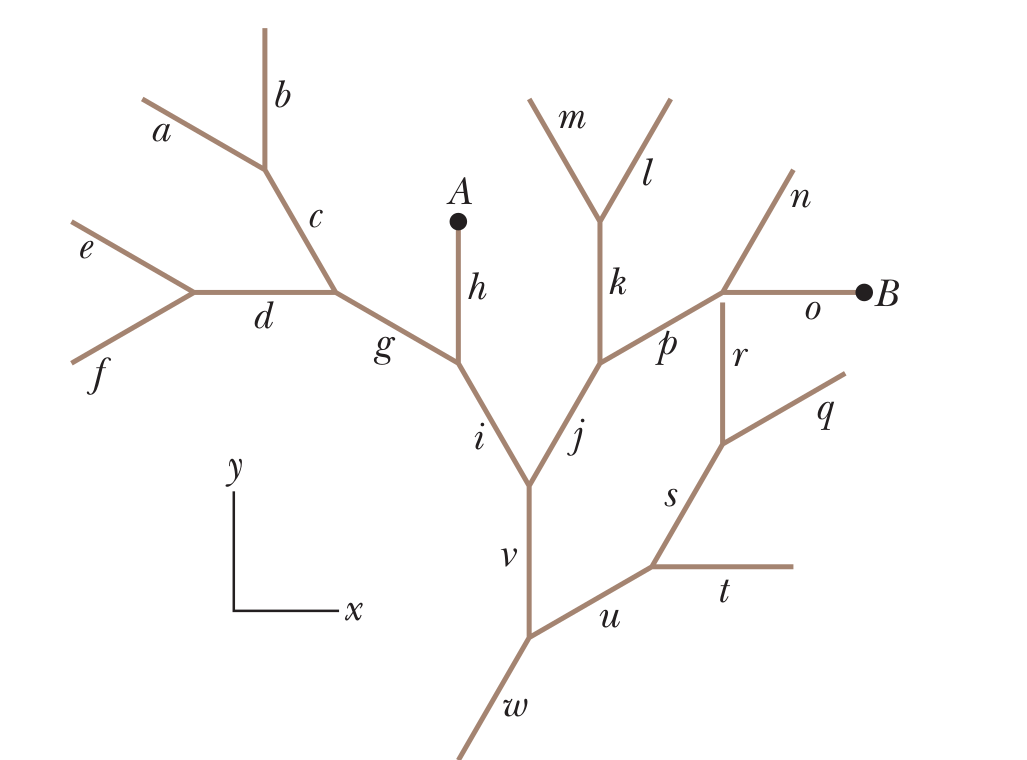
\includegraphics[width=10cm]{Exam1Practice_Figures/vector.png}
       \caption{3-29}
    \end{figure}
    \begin{subequations}
    
    \subsubsection{Solution}
    \end{subequations}

    \newpage

    \subsection{Problem 31: Page 58}
    In Fig. 3-30, a vector $\va{a}$ with a magnitude 
    of $17.0\,\mathrm{m}$ is directed at angle $\theta=56.0\degree$
    counterclockwise from the $+x$ acis. What are the 
    components (a) $a_x$ and (b) $a_y$ of the vector? A 
    second coordinate system is inclined by angle $\theta'=18.0\degree$
    with respect to the first. What are the components (c) $a'_x$ 
    and (d) $a'_y$ in this primed coordinate system?
    \begin{figure}[h!]
        \centering
        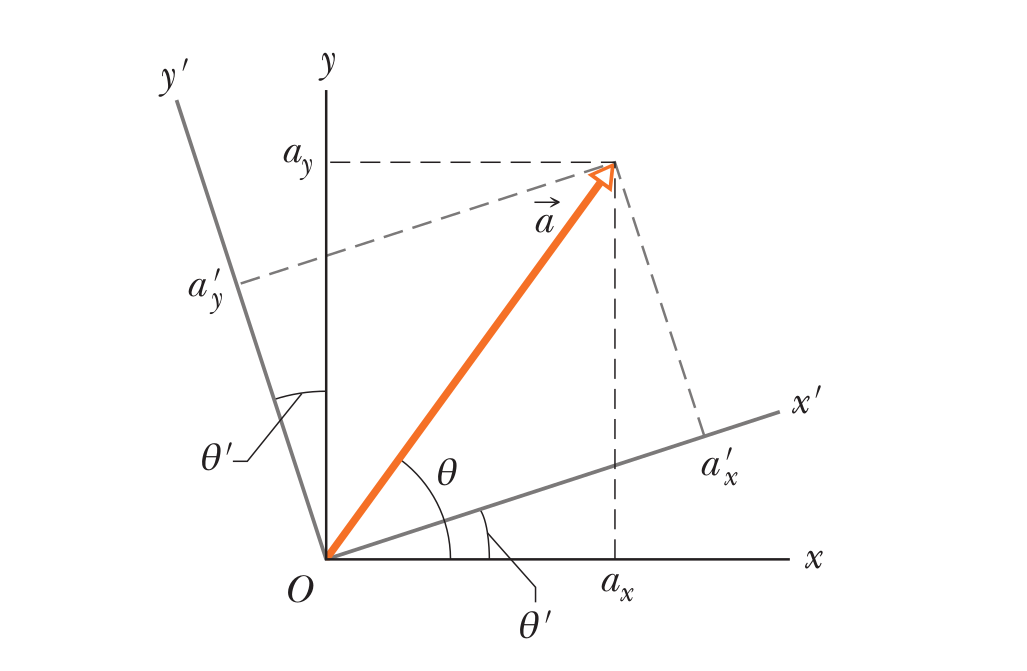
\includegraphics[width=10cm]{Exam1Practice_Figures/vector2.png}
        \caption{3-30}
    \end{figure}
    \begin{subequations}
    
    \subsubsection{Solution}
    \end{subequations}

\newpage

\section{Chapter 4: 2D and 3D Motion}

    \subsection{Problem 38: Page 86}
    A golf ball is struck at ground level. The speed of the golf 
    ball is a function of the time is shown in Fig. 4-36, where 
    $t=0$ at the instant the ball is struck. The scaling on the vertical 
    axis is set by $v_a=19\,\mathrm{m/s}$ and $v_b=31\,\mathrm{m/s}$.
    \begin{enumerate}[label=(\alph*)]
        \item How far does the golf ball travel 
        horizontally before returning to ground level?
        \item What is the maximum height above the ground 
        level attained by the ball?
    \end{enumerate}
    \begin{figure}[h!]
        \centering    
        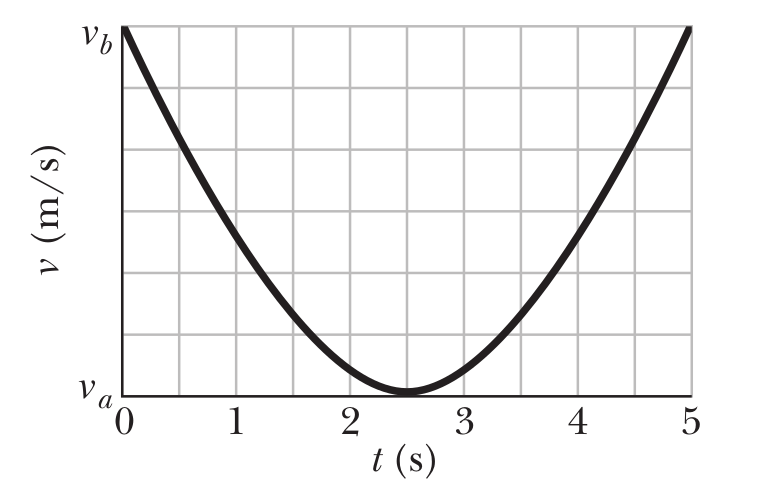
\includegraphics[width=10cm]{Exam1Practice_Figures/motion.png}
    \end{figure}
    \begin{subequations}
    
    \subsubsection{Solution}
    \end{subequations}

    \newpage

    \subsection{Problem 71: Page 88}
    A suspicious-looking man runs as fast as he can along a moving 
    sidewalk from one end to the other, taking $2.50\,\mathrm{s}$. Then 
    security agents appear, and the man runs as fast as he can back 
    along the sidewalk to his starting point, taking $10.0\,\mathrm{s}$.
    What is the ratio of the man's running speed to the sidewalk's speed?
    \begin{subequations}
    
    \subsubsection{Solution}
    \end{subequations}

\newpage

\section{Chapter 5: Force and Motion}
    \subsection{Problem 34: Page 119}
    In Fig. 5-40, a crate of mass $m=100\,\mathrm{kg}$ is 
    pushed at constant speed up a frictionless ramp ($\theta=30.0\degree$)
    by a horizontal force $\va{F}$. What are the magnitudes of:
    \begin{enumerate}[label=(\alph*)]
        \item $\va{F}$
        \item the force on the crate from the ramp?
    \end{enumerate}
    \begin{figure}[h!]
        \centering 
        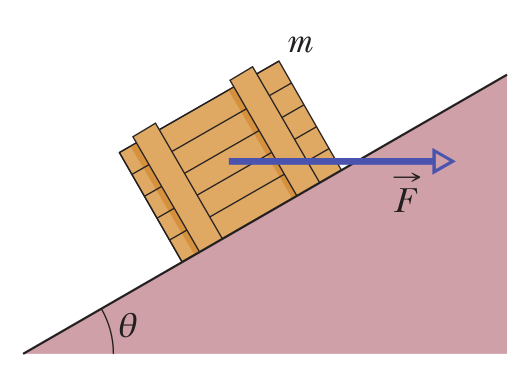
\includegraphics[width=10cm]{Exam1Practice_Figures/force.png}
    \end{figure}
    \begin{subequations}
    
    \subsubsection{Solution}
    \end{subequations}

    \newpage

    \subsection{Problem 39: Page 119}
    A sphere of mass $3.0x10^{-4}\,\mathrm{kg}$ is suspended 
    from a cord. A steady horizontal breeze pushes the sphere so that 
    the cord makes a constant angle of $37\degree$ with the vertical. Find:
    \begin{enumerate}[label=(\alph*)]
        \item the push magnitude
        \item the tension in the cord
    \end{enumerate} 
    \begin{subequations}
    
    \subsubsection{Solution}
    \end{subequations}

    \newpage

    \subsection{Problem 40: Page 119}
    A dated box of dates, of mass $5.00\,\mathrm{kg}$, is sent 
    sliding up a frictionless ramp at an angle of $\theta$ to 
    the horizontal. Figure 5-41 gives,
    \begin{figure}[h!]
        \centering 
        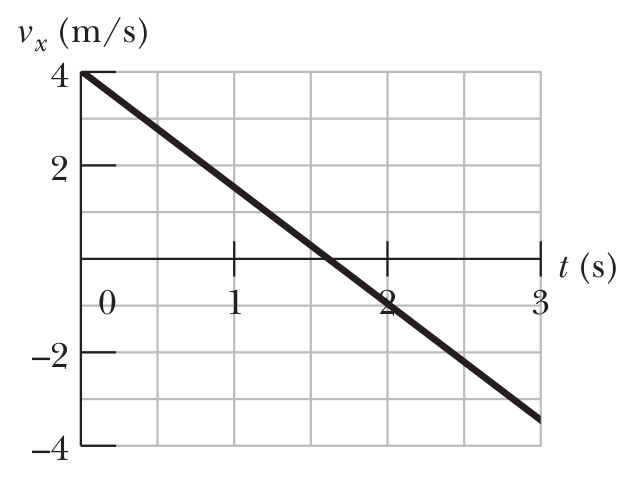
\includegraphics[width=10cm]{Exam1Practice_Figures/force2.png}
        \caption{5-41}
    \end{figure}
    as a function of time $t$, the component $v_x$ of the box's velocity 
    along an $x$ axis that extends directly up the ramp. What is the magnitude 
    of the normal force on the box from the ramp?
    \begin{subequations}
    
    \subsubsection{Solution}
    \end{subequations}

\end{document}